%
\section{Introduction}
\label{sec:intro}


\IEEEPARstart{B}{uilding} extraction, which aims to extract building regions in a high resolution satellite image, remains as one of the fundamental challenges in the field of remote sensing.
Extraction of building rooftops from aerial and satellite imagery is an important step in many applications, such as urban planing, automated map making, 3D city modeling, updating geographical dataset, and so on.
However, it is particularly challenging to automatically extract rooftops at the pixel level for the following reasons:
%
\begin{itemize}
 \item Different density of buildings in different type of scenes. A rural scene has low density, while an urban scene has high density, and a suburban scene has medium density in between.
 \item Diverse shapes of the buildings. Buildings appear in a wide range of shapes, varying from simple rectangular blocks with flat roof to complex shapes with intricate roof shapes.
 \item The quality of remote sensing images. Images vary in terms of contrast, resolution, and image principle \cite{IEEEexample:huertas1988detecting}. \cxj{Do we have problem with image qualities? Or do you have experiments on that?}
\end{itemize}
%

We show several typical patches of satellite images in Fig.~\ref{fig:intro} to illustrate the above challenges in the building extraction task.
\fymd{Fig.~\ref{fig:intro}(a) shows that the back face of the roof covered in shadow. And Fig.~\ref{fig:intro}(b)(c) demonstrates the variance between and within different classes. Additionally, the dense and tiny buildings are presented in Fig.~\ref{fig:intro}(d).}

\begin{figure}
\centering
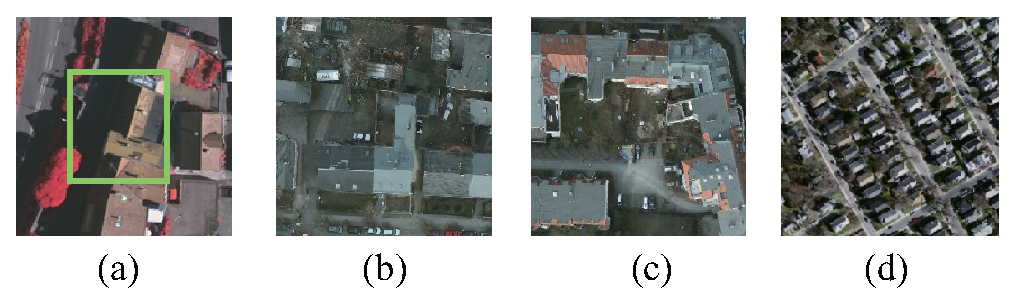
\includegraphics[width=8.7cm]{Figures/challenge.eps}
\caption{Examples of satellite image patches with different kinds of challenges. (a) Shadow occlusion in green frame. \cxj{But you only extract building roofs..So the shadow is good for large contrast.}(b) Low inter-class differences. (c) High intra class variance. (d) A large amount of tiny and dense buildings.}
\label{fig:intro}
\end{figure}


In the past decades, many researchers have made enormous effort to extract buildings automatically from satellite images.
At first, many simple knowledge-based methods were put forward~\cite{IEEEexample:huertas1988detecting,IEEEexample:noronha2001detection,IEEEexample:nosrati2009novel, IEEEexample:izadi2012three,IEEEexample:wang2015efficient}.
Their basic ideas are derived from prior knowledge that buildings are closed polygons made up of some straight lines.
Some others are energy-based methods including the variational level set evolution, improved snake model and graph cut \cite{IEEEexample:cote2013automatic, IEEEexample:peng2005improved,IEEEexample:sirmacek2009urban}.
Due to that early methods depend heavily on prior knowledge and initialization, they do not work well for building extraction of complex scenes.


In recent years, with the development of machine learning, many \xjmd{deep-learning-based} techniques are gradually introduced into the remote sensing area.
At first, some shallow networks were proposed for multiple geographic object extraction~\cite{IEEEexample:mnih2013machine, IEEEexample:saito2016multiple,IEEEexample:alshehhi2017simultaneous,IEEEexample:zhao2017contextually}.
These methods typically use image patches with a fixed size \fymd{feeded into a shallow CNNs} for segmentation, they are not efficient or accurate enough for the pixel-wise segmentation task for large-scale satellite images.
\cxj{Do these method use deep learning or just machine learning?}
%
Later on, with the rapid growth of computational powers, deep learning technology developed rapidly and some researchers tried deep learning for aerial images classification and semantic pixel labeling~\cite{IEEEexample:paisitkriangkrai2015effective,IEEEexample:liu2017dense,IEEEexample:audebert2017deep,IEEEexample:kampffmeyer2017urban,IEEEexample:he2017multi}.
Unfortunately, while ignoring the hierarchical information extracted by the network, they could not deal with the scenes which contains close-packed buildings well.



This paper propose a relatively simple, but very effective strategy for fusing
multi-scale features in neural networks.
It could be combined with a general CNN architecture easily for robust building extraction.
Differ from above mentioned methods, we take full advantages of \emph{the low-level appearance information as well as high-level semantic information} by the novel fusion operation in a way of stage by stage.
Inspired by the FCN~\cite{IEEEexample:Long_2015_CVPR}, whose output is in the same resolution of its input, we propose a novel hierarchically fused FCN, named HF-FCN for buildings pixel-wise classification.
Differ from the traditional FCN, a set of hierarchical fusion operations are used to fuse the intra layer information and inter layer information respectively which improve the performance of FCN greatly.
And numerous experiments conducted on three remote sensing image datasets all obtain fairly good results.
Further, \fymd{we integrate our method into the pipeline of building reconstruction as the part of building detection.}
\cxj{3d modeling is not part of building detection.}
\cxj{Do you have any quantitative measure for the quality of 3D reconstruction?}

Overall, our technical contributions are:
%
\begin{enumerate}
	\item We propose an effective hierarchical fusion strategy which is specially designed for multi-scale building extraction in high-resolution satellite images. Combining with a generic FCN, a novel network is presented, named HF-FCN that can deal with the problems of different sizes, diverse appearance and mutual occlusion of buildings and etc.
	\item HF-FCN is an end-to-end network that does not need any post processing. The approach is much more computationally efficient than existing techniques. Besides, the overall accuracy of the proposed HF-FCN exceeds the state-of-art algorithms.
	\cxj{Do you compare with recent papers?}
\end{enumerate}

The remainder of this paper is organized as follows. Sec.~\ref{Sec:RelatedWork} sums up the related works in the past.
In Sec.~\ref{Sec:HF-FCN}, we introduce the fusion operation and architecture of HF-FCN, as well as the training details.
In Sec.~\ref{Sec:exp}, a brief description of the dataset used for our task is provided. HF-FCN training strategies, details and its evaluation metrics are also described.
In Sec.~\ref{Sec:Res}, we display and analysis the experimental results.
Extension in 3D building modeling are presented in Sec.~\ref{sec:app}.
Finally, the conclusion is discussed in Sec.~\ref{Sec:Con}.
